\section{Diagramas de estados}
Para especificar os principais processos do projeto foram então desenvolvidos diagramas de estados,
sendo então pretendido demonstrar o processo de criação de um tópico do fórum por parte de um técnico, o 
processo de aceder e responder a um tópico e o login com ativação de conta
visto que estas interações são as de maior significância e regradas no software.

\subsection{Diagrama de estados criação de tópico}

Com o diagrama de estados de criação de tópico é pretendido demonstrar o processo de criação de um tópico 
por parte de um técnico. Assim sendo este primeiramente terá de estar autenticado, caso não esteja 
este será encaminhado para autenticação. De seguida criará tópico, após preencher os 
campos desejados este poderá confirmar o tópico, caso confirme é verificado se o tópico possui título, 
caso não possua, é invalido pelo que o técnico deverá preencher os dados em falta, caso o 
título esteja preenchido é verificado se possui descrição e tipo, caso não possua é seguido o mesmo fluxo que o 
caso anterior, caso contrário é criado um tópico. Se o técnico não desejar confirmar o tópico ele 
poderá cancelar, quando assim o faz este torna-se cancelado.

\begin{figure}[htb]
    \centering
    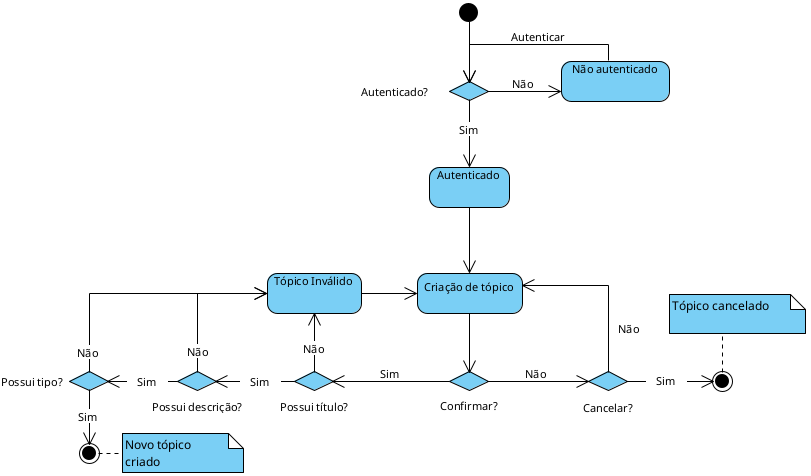
\includegraphics[width=0.9\textwidth]{images/diagramas/estados/criar_topico.png}
    \caption{Diagrama de estados de criar tópico}
    \label{fig:27}
\end{figure}

\newpage

\subsection{Diagrama de estados responder a tópico}

Com o diagrama de estados de responder a tópico é pretendido demonstrar o processo de seleção e 
responder a um tópico por parte de um técnico. Assim sendo que o técnico primeiramente deverá estar 
autenticado, caso não esteja este será encaminhado para a autenticação. Após a autenticação o técnico 
estará autenticado e irá por predefinição ver tópicos em destaque, nesta listagem este selecionará um 
tópico ficando assim o tópico 
selecionado. Assim que o tópico se encontra selecionado o técnico conseguirá responder a este criando 
um comentário. Após a criação do comentário este poderá confirmar o comentário, caso confirme o 
comentário ficará criado, caso contrário este comentário ficará cancelado.

\begin{figure}[htb]
    \centering
    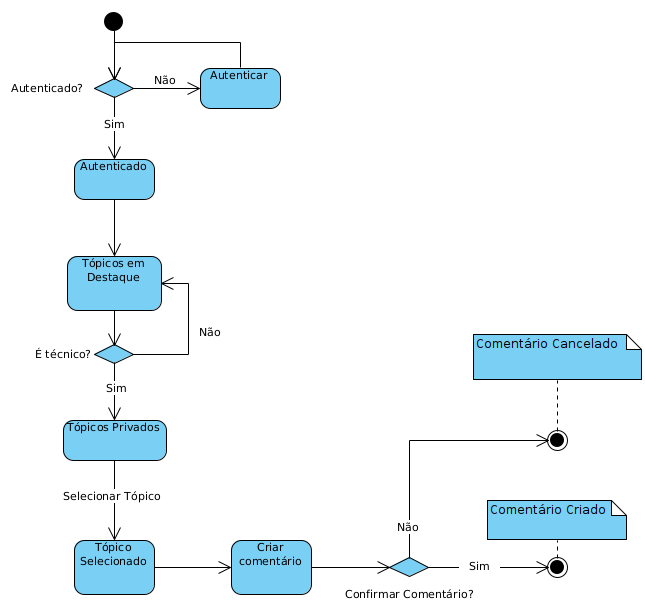
\includegraphics[width=0.7\textwidth]{images/diagramas/estados/responder_topico_tecnico.png}
    \caption{Diagrama de estados de criar tópico}
    \label{fig:28}
\end{figure}

\newpage

\subsection{Diagrama de estados autenticação e validação de conta}

Assim que o técnico decide realizar o login na aplicação este indica as suas credenciais, caso estas 
credenciais não estejam corretas, a autenticação será incorreta e deverá alterar as credenciais. 
Caso as credenciais estejam corretas e a conta válida o técnico ficará autenticado, caso contrário o 
este terá uma conta inválida, pelo que deverá ser validada, para  isso o este deverá 
inserir o código de validação, se o código estiver correto, a conta será validada e o técnico 
ficará autenticado, caso contrário o código será invalido e o deverá indicar o seu código de 
validação novamente.

\begin{figure}[htb]
    \centering
    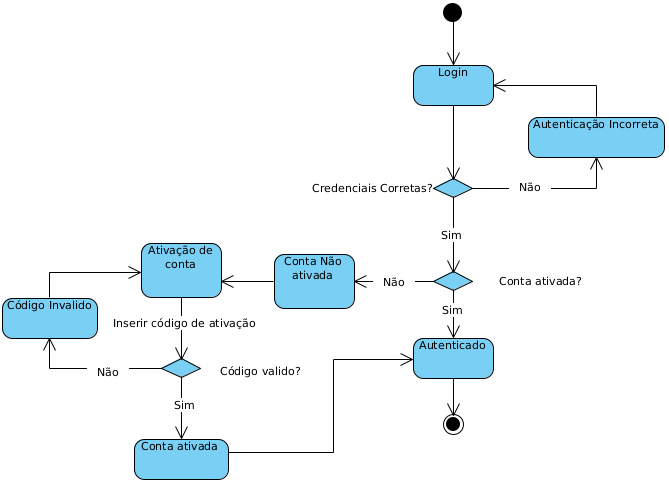
\includegraphics[width=0.7\textwidth]{images/diagramas/estados/autenticacao.png}
    \caption{Diagrama de estados de autenticação e validação de conta}
    \label{fig:29}
\end{figure}
